%%%%%%%%%%%%%%%%%%%%%%%%%%%%%%%%%%%%%%%%%
% Short Sectioned Assignment
% LaTeX Template
% Version 1.0 (5/5/12)
%
% This template has been downloaded from:
% http://www.LaTeXTemplates.com
%
% Original author:
% Frits Wenneker (http://www.howtotex.com)
%
% License:
% CC BY-NC-SA 3.0 (http://creativecommons.org/licenses/by-nc-sa/3.0/)
%
%%%%%%%%%%%%%%%%%%%%%%%%%%%%%%%%%%%%%%%%%

%----------------------------------------------------------------------------------------
%	PACKAGES AND OTHER DOCUMENT CONFIGURATIONS
%----------------------------------------------------------------------------------------

\documentclass[paper=a4, fontsize=11pt]{scrartcl} % A4 paper and 11pt font size

\usepackage[T1]{fontenc} % Use 8-bit encoding that has 256 glyphs
\usepackage{fourier} % Use the Adobe Utopia font for the document - comment this line to return to the LaTeX default
\usepackage[english]{babel} % English language/hyphenation
\usepackage{amsmath,amsfonts,amsthm} % Math packages

\usepackage{graphicx}

\usepackage{sectsty} % Allows customizing section commands
\allsectionsfont{\centering \normalfont\scshape} % Make all sections centered, the default font and small caps

\usepackage[procnames]{listings}

\usepackage{fancyhdr} % Custom headers and footers
\pagestyle{fancyplain} % Makes all pages in the document conform to the custom headers and footers
\fancyhead{} % No page header - if you want one, create it in the same way as the footers below
\fancyfoot[L]{} % Empty left footer
\fancyfoot[C]{} % Empty center footer
\fancyfoot[R]{\thepage} % Page numbering for right footer
\renewcommand{\headrulewidth}{0pt} % Remove header underlines
\renewcommand{\footrulewidth}{0pt} % Remove footer underlines
\setlength{\headheight}{13.6pt} % Customize the height of the header

\numberwithin{equation}{section} % Number equations within sections (i.e. 1.1, 1.2, 2.1, 2.2 instead of 1, 2, 3, 4)
\numberwithin{figure}{section} % Number figures within sections (i.e. 1.1, 1.2, 2.1, 2.2 instead of 1, 2, 3, 4)
\numberwithin{table}{section} % Number tables within sections (i.e. 1.1, 1.2, 2.1, 2.2 instead of 1, 2, 3, 4)

\setlength\parindent{0pt} % Removes all indentation from paragraphs - comment this line for an assignment with lots of text

%----------------------------------------------------------------------------------------
%	TITLE SECTION
%----------------------------------------------------------------------------------------

\newcommand{\horrule}[1]{\rule{\linewidth}{#1}} % Create horizontal rule command with 1 argument of height

\title{	
\normalfont \normalsize 
\textsc{BRSU} \\ [25pt] % Your university, school and/or department name(s)
\horrule{0.5pt} \\[0.4cm] % Thin top horizontal rule
\huge Neural Networks\\Assignment 7 \\ % The assignment title
\horrule{2pt} \\[0.5cm] % Thick bottom horizontal rule
}

\author{Bastian Lang} % Your name

\date{\normalsize\today} % Today's date or a custom date

\begin{document}

\maketitle % Print the title

\newpage

\section{Outline}

\section{PCA \& ICA}

\subsection{output}
\begin{figure}[ht]
	\centering
  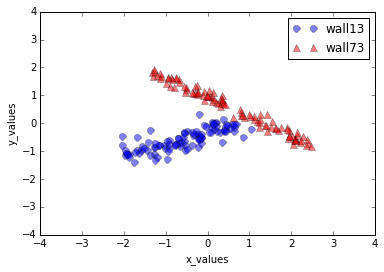
\includegraphics[width=0.8\textwidth]{combined.png}
	\caption{Both datasets in new coordinate system after performing PCA.}
	\label{fig1}
\end{figure}

\subsection{code}
\begin{lstlisting}
# -*- coding: utf-8 -*-
"""
Created on Sat Nov 21 12:41:57 2015

@author: bastian
"""

from matplotlib.mlab import PCA as mlabPCA
import matplotlib.pyplot as plt
import numpy as np

def do_pca(data, class_label):
    
    mlab_pca = mlabPCA(wall13_data)
    
    
    print('PC axes in terms of the measurement axes scaled by the standard deviations:\n', mlab_pca.Wt)
    
    # pca
    plt.plot(mlab_pca.Y[:,0],mlab_pca.Y[:,1],
             'o', markersize=7, color='blue', alpha=0.5, label=class_label)
    # original
    plt.plot(wall13_data[:,0], wall13_data[:,1],'^', markersize=7, color='red', alpha=0.5, label='original')
    
    plt.xlabel('x_values')
    plt.ylabel('y_values')
    plt.xlim([-4,40])
    plt.ylim([-4,10])
    plt.legend()
    plt.title('Transformed samples versus original data')
    
    plt.show()



wall13_data = np.genfromtxt('wall13.csv', delimiter=',')
do_pca(wall13_data, 'wall13')

wall73_data = np.genfromtxt('wall73.csv', delimiter=',')
do_pca(wall73_data, 'wall73') 



def split_pca(combined_data, label_1, label_2):
    
    mlab_pca = mlabPCA(combined_data)
    
    print('PC axes in terms of the measurement axes scaled by the standard deviations:\n', mlab_pca.Wt)
    
    plt.plot(mlab_pca.Y[0:100,0],mlab_pca.Y[0:100,1],
             'o', markersize=7, color='blue', alpha=0.5, label=label_1)
    plt.plot(mlab_pca.Y[100:200,0], mlab_pca.Y[100:200,1],
             '^', markersize=7, color='red', alpha=0.5, label=label_2)
    
    plt.xlabel('x_values')
    plt.ylabel('y_values')
    plt.xlim([-4,4])
    plt.ylim([-4,4])
    plt.legend()
    plt.title('Transformed samples with class labels from matplotlib.mlab.PCA()')
    
    plt.show()
    

mixed_data = np.concatenate((wall13_data, wall73_data), axis=0)
split_pca(mixed_data, 'wall13', 'wall73')
\end{lstlisting}



\end{document}